\section{Digital Design Overview}

The digital system of the Q-Pix readout begins when the first digital data are recorded.
This occurs during the collection of a recorded timestamp in response to the logic reset pulse sent from the integrating analog front-end.
This record happens in response to output reset-pulse sent from any one, or more, of the pixels.
Then, the timestamp record is the value of a local 32-bit counter at the time the node receives the reset pulse.
When a reset occurs the data recorded are the reset values of each pixel, and the only data required for a full analysis of all reconstruction with a LArTPC are:

\begin{figure}[]
\centering
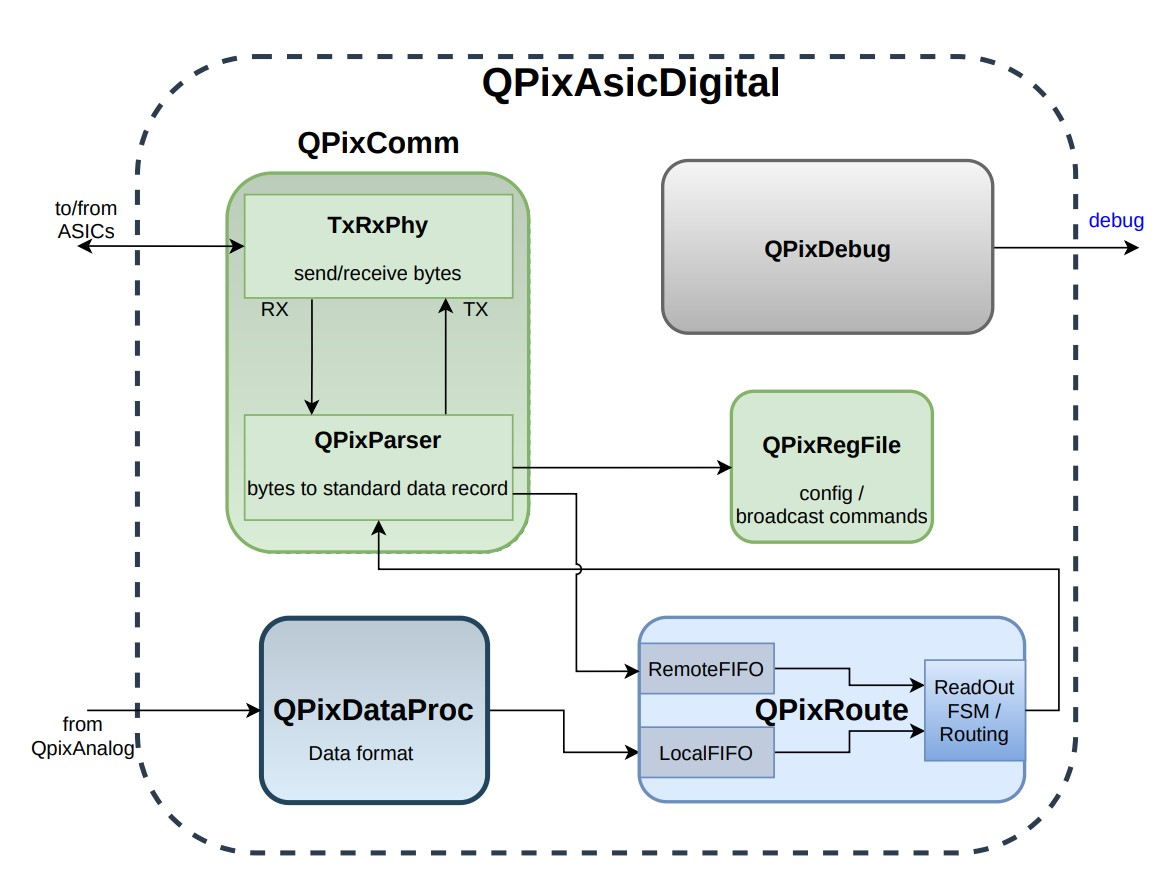
\includegraphics[width=\textwidth]{images/digital_node_overview.jpg}
\caption{Diagram of the Digital node.
  The controlling sections of the logic for the digital node are QpixComm, QPixDataProc, QPixRoute, and QPixRegFile.
  The Comm layer is responsible for routing packets between the physical layer and handles the parsing of incoming data packets.
  The DataProc layer is responsible for recording timestamp data during a reset from the analog front-end.
  The RegFile contains configuration information, such as routing.
  QPixRoute determines the controlling state machine that, based on register configurations, determines what packets are sent to which neighboring nodes.}
\end{figure}~\label{fig:qpa_diagram}

Each of these remote ASICs are running on free-running independent clocks, designed with a frequency of 30~\unit{MHz}.

\subsection{Communications}~\label{sec:digi_communications}

The QpixComm module controls incoming and outgoing packet logic.

The logic responsible for indentifying how an incoming packet is handled is defined in QPixParser.
When a valid 64 bit packet has been received, a valid signal is thrown high.
The packet is handled based on the bits within the header of this packet.
How the packet is handled is determined the by the packet header~\ref{bit_reservation}.

Packets are only comprehensable for types if the same region of the 64 bits are ubiqutous.
For this purpose all packets use or reserve the same 20 bits, with four bits reserved for the packet type:

\begin{itemize}
    \item Unused, 60--63
    \item Header, 56--59
    \item X Location, 36--39
    \item Y Location, 32--35
\end{itemize}~\label{bit_reservation}

If the packet originated from the aggregator node then this packet is treated as a broadcast.
Broadcast commands record unique numbers associated with this request and are also sent to all connected neighbornoods except from the direction that the broadcast is received.
A unique broadcast number is used to avoid registering the same request.

If the packet was not from an aggregator node, then this packet is treated as remote data from a neighbor node.
All data transfers of any kind are treated so that all communication happens between individual nodes and an aggregator node.
Therefore, any packet that originates on a node that isn't the aggregator node will be sent to the aggregator node.
The direction of that this packet is sent is deteremined by a configuration register.

\subsection{The Structure of a Data Word}

Each digital node responds to a successful transmission of a 64-bit packet.
We choose that each packet, regardless of type, be 64-bits to reduce the overall packet checking complexity on each node.
The type of the packet then is selected by the word type, which is reserved for a static 4 bits within each 64-bit word.
This allows for a total amount of 16 unique packets each of which may be handled differently.

A successful transmission of a data word is indicated by the protocol when the correct number of bits have been read~(see Section~\ref{sect:endeavor}).
When a correct packet is filled a single flag is raised to indicate that the word is valid, and then the appropriate logic parses the header bits of the packet and determines how the packet should be handled.

There are two main types of packets that a digital node would receive, a register request or a data word from another node.
In the first case, the register request indicates that this packet originated from the aggregator node and may either to a specific node or a broadcast to the entire array.
Whether or not the register request is a broadcast is checked against another bit, and the packet is handled accordingly.
If the packet is a broadcast, the receiving node records an identification number associated with the broadcast, which it uses to ignore additional packets it may receive that correspond to the same broadcast.

The second kind of packet the digital node may receieve is a data type word.
In the case of data words, there are also two main types: a word which contains the 32 bit timestamp or an event end word.
The 32 bit timestamp data word are the words which must eventually make it to disk for analysis.
The data words must also encode the row and column position of the original nodes.

\subsection{Configuration}

The configuration of the digital node is handled through local registers.
These registers are described within QpixRegFile module, shown in Figure.~\ref{fig:qpa_diagram}.
These registers include the ability to control routing of data packets, reset, enable, and channel masking.
The Table~\ref{tab:registers} describes the implemented register addresses and their functions:

\begin{table}
\begin{center}
\begin{tabular}{||c c c||}
 \hline
 Address & Name & Function \\ [0.5ex]
 \hline\hline
  0x01 & Command & Used to broadcast type or trigger \\
 \hline
  0x03 & Routing & Allows selection between manual or dynamic routing. \\
 \hline
  0x04 & Channel Mask & Selection of mask prevents triggers from masked channels. \\
 \hline
  0x05 & Position & Allows configuration of X and Y coordinates of node. \\
 \hline
  0x06 & Disable & Selection of which neighboard node inputs are ignored. \\
 \hline
  0x08 & Local Disable & Selection of which input and out neighboard nodes can be ignored. \\
 \hline
\end{tabular}
\caption{The address values are not sequential because some registers have become deprecated through development.}
\end{center}
\end{table}
~\label{table:node_registers}

The composition of any register word is shown in Table~\ref{tab:packet_register}.
\begin{table}
\begin{center}
\begin{tabular}{|| p{30mm} | p{30mm} | p{90mm} ||}
 \hline
 Bit Location & Name & Function \\ [0.5ex]
 \hline\hline
  0--15 & Data & Excess bits  \\
 \hline
  16--31 & Address & Excess bits  \\
 \hline
  40--43 & Y Position Transfers & Next Y position in tile. \\
 \hline
  44--47 & X Position Transfers & Next X position in tile. \\
 \hline
  48 & Source Flag & Single Bit flag to indicate whether ot not packet originated from aggregator. \\
 \hline
  49--52 & Request ID & Identifier bits to specify broadcast. \\
 \hline
  53 & Destination Flag & Identifier bit to specify if broadcast is meant for a specific node. \\
 \hline
  54 & Read Flag & Identifier flag to specify if register request is a read. \\
 \hline
  55 & Write Flag & Identifier flag to specify if register request is a write. \\
 \hline
\end{tabular}
\caption{Description of the bit values within the register request word.}
\end{center}
\end{table}
~\label{tab:packet_register}

\subsection{Local Data Collection}

The digital node is responsible for collecting and storing local timestamps in response to pixel resets as well as being able to communicate these data with neighbor nodes.
The node must be able to buffer data so as to prevent packet loss during transactions.
The separation of the remote and local packets are contained within two different FIFOs, as shown in Figure.~\ref{fig:qpa_diagram}.

There are two conditions which must be met in order for a timestamp to be recorded.
First, an incoming reset pulse must be supplied from one of the pixels.
Second, at the time of this incoming reset the corresponding pixel mask must not be set in the channel mask register (See Table~\ref{table:node_registers}).
When both conditions the value of the local reset is recorded into a 32 bit wide FIFO shown in QpixRoute in Figure~\ref{fig:qpa_diagram}.

The composition of the data word is shown in Table~\ref{tab:packet_register}.
\begin{table}
\begin{center}
\begin{tabular}{|| p{30mm} | p{30mm} | p{90mm} ||}
 \hline
 Bit Location & Name & Function \\ [0.5ex]
 \hline\hline
  0--31 & Timestamp & Basic Datum which records the local counter at the time of the reset pulse. \\
 \hline
  32--35 & Y Position & Assigned Y position in tile. \\
 \hline
  36--39 & X Position & Assigned X position in tile. \\
 \hline
  40--55 & Pixel Mask & Pixels which were issuing a reset at this time. \\
 \hline
  56--59 & Word Header & Header value, which is commond to all packets. \\
 \hline
  60--63 & Reserved & Unused bits for all packets. \\
 \hline
\end{tabular}
\caption{Data word composition.}
\end{center}
\end{table}
~\label{tab:packet_data}

\subsubsection{The Local Data Packet}~\label{sec:local_data_packet}

The transmission of the reset data from the local FIFO to adjacent neighbor nodes begins when an incoming register request from the aggregator is received.
This request is supplied as register request to the command register (~\ref{table:node_registers}).
This request may be considered either a ``hard'' or a ``soft'' interrogation command.

The difference between the two types of an interrogation command is whether or not the event end packet is created.
In the case of a ``hard''--interrogation, the event end packet is always created, regardless of the local FIFO.
In the case of a ``soft''--interrogation, the event end packet is created only if the local FIFO is not empty.

The use of two different types of interrogations allows the aggregator control flexibility in how many packets are created during an interrogation.
Interrogations may happen on timescales much more quickly than expected resent pulses ($\mathcal{O}(10^{1}~\unit{s})$, Chapter~\ref{chapters/qpix.tex}).
The ability to request data only if available prevents an over abundance of packets which prevents needless data transfers, reduces remote FIFO buildup, and conserves power.

\subsubsection{The Event End Packet}

The event end words perform multiple functions.
First, they may used as checksums to indicate at the aggregator node, or on disk, that this node has successfully transmitted all of its data.
Secondly, the event end word, since it is necessarily 64 bits long, may also transmit its own timestamp with the excess bits.
The timestamp that the event end word carries is the time that the time that the node received the broadcast.
This timestamp is used in the frequency calibration of the node; the method for calibration is described in greater detail in Section~\ref{sec:calib}.

\subsection{Debug and Future ASIC Prototypes}

Finally, The last block in Figure.~\ref{fig:qpa_diagram} is the QPixDebug.
This portion is is used to expose certain ports to the physical pins in a digital ASIC design.
This design will be the first prototype of the digital ASIC, and is beyond the scope of the work presented here, but will be discussed in the final section of this thesis.

\subsubsection{Inter-Node communication via endeavor protocol}
~\label{sect:endeavor}

The Endeavor protocol is a bi-directional serial communication protocol which allows communication between asynchronous devices.
The asynchronous communication is achieved by extending the length of time that each bit is sent between the two devices.
In this protocol the way that the receiving node (RXN) identifies the correct logic value of the current bit is by counting the number of clocks that the incoming signal is logic high.
The incoming bit is either a logic low, if held high for fewer clocks than it would be if it was an incoming logic high.
The number of clocks which corresond to high and low must be programmed beforehand and are tunable parameters.

\begin{figure}[]
\centering
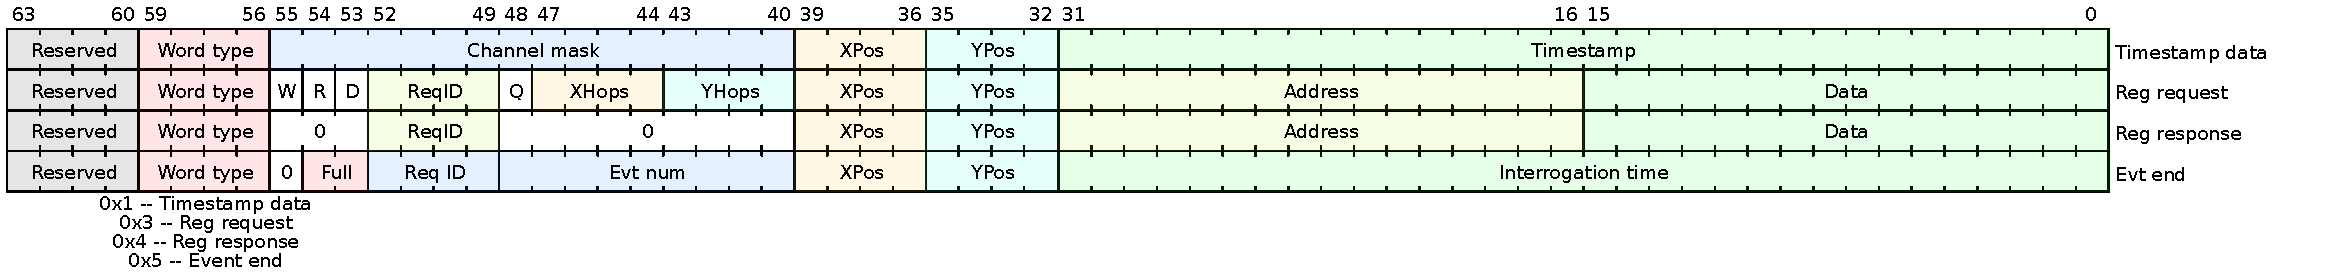
\includegraphics[width=\textwidth]{images/qpix_word_format.pdf}
\caption{Example of Datum words and their allocation as currently implemented in the simulation and first prototypes.}
\end{figure}~\label{fig:datum}

\subsection{Basic System Requirements}

The sheer number of pixels required for an APA (and the 10~\unit{kT} entire module) require an effective means of charge and time calibration, stable buffer depths, and protection against single-point failure (SPF).
Resets are records of a local counter at the current node and are recorded in response to a reset pulse sent from a pixel.

\subsubsection{Comments on Data Rates and required Computing}

Based on the minimum number of bits for each RTD~\ref{bit_calc} we can estimate minimum data rates based on tile size.


\section{The Digital Finite State Machine}~\label{sec:digital_fsm}

The Finite State Machine (FSM) of the digital ASIC outlines the designed behavior response to input.
Figure~\ref{fig:digital_fsm} shows a representation of the different states as well as the conditions to enter or leave each state.

There are two different kinds of prompts that an ASIC can receive: packet transactions from neighbors and resets from pixels.
When an ASIC receives a packet from a neighbor, the packet data are written on the remote FIFO
There is one special packet


\begin{figure}[]
\centering
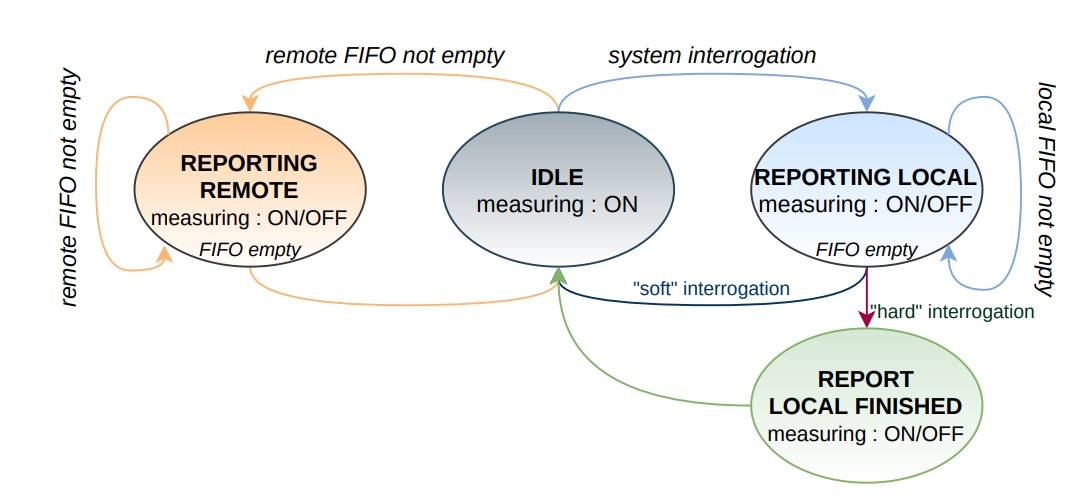
\includegraphics[width=\textwidth]{images/digital_fsm_overview.jpg}
\caption{Diagram of the Digital node's FSM which determines how to respond to incoming packets.}
\end{figure}~\label{fig:digital_fsm}

\begin{itemize}
    \item Idle, Acquisition State
    \item Transmit Local
    \item Transmit Finish
    \item Transmit Remote
    \item DONE
\end{itemize}~\label{fsm_state_labels}

\subsection{Idle}~\label{sec:state_idle}

\subsection{Transmit Data}~\label{sec:state_data}

\subsection{Transmit Remote}~\label{sec:state_remote}


\section{The Parameter Space of the Digital System}~\label{sec:parameter_space}

The digital back-end design

\subsection{Buffer Depth Requirements}

The required buffer depth of each node in an array is the maximum number of timestamps the node can store in memory before overflow (dataloss).
Each node requires some buffer memory to record local data as well as separate storage for remote data.
The remote data which can be sent can come from any of the adjacent connected nodes, and may of any type: data words, register request, etc.
Since the remote

The ice40 FPGAs have a total of 20 Embedded Block Ram models (EBRs) which allow for a for total of 64xTODO memory depths allocated in each node.

\subsection{Endeavor Packet Stability at Different Scales}

We test two differet scales for the endeavor protocol.
This protocol maintains a relative relationship between the number of high signals used to send either a high and low bit.
The convention to send a high bit is to pulse a logic high signal for twice as long as is done for a low bit.

The number of bits used for to send a high bit are either

\begin{table}
\begin{center}
\begin{tabular}{||c c c||}
 \hline
 Name & Function & Value Range\\ [0.5ex]
 \hline\hline
  Zero & Controls how many clocks to send a logic high to transfer a low bit & 1--3 \\
 \hline
  One & Controls how many clocks to send a logic high to transfer a high bit & 2--5 \\
 \hline
\end{tabular}
\caption{The address values are not sequential because some registers have become deprecated through development.}
\end{center}
\end{table}
~\label{table:endeavor_bits}

\subsection{The Push and Pull Architectures}~\label{sec:architectures}


\section{The Digital Back-end problem}

The main objectives of the digital back-end are to correctly measure the data presented to it by the analog front-end and ensure lossless transport of that data to disk.
More simply, the goals of the digital portion of the Q-Pix readout are to record and send data.
We note that the successful completion of these two objectives to be goal of these simulation studies.

\subsection{The Basic Datum}

We begin with a discussion of the basic datum and mention initial design choices at the physical connection interface.
The structure of this datum determines the buffer widths and depths required to store the data at the local ASIC level as well as the protocol used to transfer this data between ASICs and eventually out of the detector.

The minimum data which needs to be recorded are the timestamp, the relative location of the digitizing ASIC within the detector, plus any channels which were responsible for this reset.
Each of the number of bits assigned to recording these parameters are a design consideration.
We choose the number of bits for the timestamp ($N_{T}$) to be 32, which prevents frequency wrap-around based on a fast clock frequency (Equation~\ref{{eq:tloop}}).
We choose as the number of bits to assign a location ($N_{loc}$) to be 8, which provides a maximum possible number of unique positions before aggregation to be 256.
Next, since the number of pixels (required by analog front-end design) is 16 we choose this number as the number of bits to represent a ``mask'' ($N_{bits} = 16$).
We need to record all of the channels during each reset since it is technically possible (even if less likely) for multiple analog channels to provide a reset within the same clock window.

We calculate the minimum number of bits per datum to be:
\begin{equation}
  N_{bits} = N_{T} + N_{pix} + N_{loc} = 32 + 16 + 8 = 56
\end{equation}~\label{eq:nbits_datum}

Since buffer memory addresses and widths are normally characterized by powers of two, we can construct the basic datum size above the minimum number of bits provided by~\ref{eq:nbits_datum} to get $N_{datum} = 64$.
The remaining bits are useful for constructing different types of packets to be used by the digital ASICs for additional uses such as register configuration or to provide packet identification.

\subsection{Communication of the Datum}~\label{sec:comms}

There exist many asynchronous protocols of communication of digital information.
Most of the differences between protocols exist based on the number of connections between devices and whether or not one pin is allocated to share a clock, etc.

Our design considerations for this readout include reduction of SPF risk, low power, and minimal routing.
Partly for these reasons, the design choice for communication relies on only two connections between ASICs.
One connection is defined as a data receiver (Rx) and the other as a data transmitter (Tx).
This choice of interface dramatically limits a choice of possible protocols.
Here, we describe the difference between two that we tested: Universal Asynchronous Receiver-Transmitter (UART) and Endeavor.
We discuss and test only these two protocols for simplicity, and find it instructive to compare a proven and custom protocol (Endeavor) with a very common one (UART).

The importance of choosing a correct protocol is to ensure lossless data transmission.
Since there are free running clocks, an asynchronous communication protocol is required.
The way to ensure that data can be moved between clocks of different speeds is to stretch the signal or to repeat bits.
The more the word is stretched in time, the larger the allowable difference in frequency between the two devices.
However, this lengthening can't proceed forever, obviously, otherwise data transmission time could exceed data capture rates.

It is another important design consideration, then, to ensure that transactions proceed as quickly as possibly without data loss.
Additional concerns of long data transactions include the use of more clock cycles which use more power and increase the risk noise to leak to the analog front-end.

%% appendix??
% \subsubsection{UART}~\label{sec:uart}
% This common protocol is typically stable between devices with a maximum difference of clock frequency to be 10\%.

% \begin{tikztimingtable}[%
%     timing/dslope=0.1,
%     timing/.style={x=5ex,y=2ex},
%     x=5ex,
%     timing/rowdist=3ex,
%     timing/name/.style={font=\sffamily\scriptsize}
% ]
% \centering
% % \busref{$CLK_{base-tx}$} & 0.10L 156{.1428570c} \\
% % \busref{$CLK_{base-rx}$} & 0.35L 156{0.12857c} \\
% \busref{$CLK_{tx}$} & 0.10L 20{c} \\
% \busref{$CLK_{rx}$} & 0.35L 22{0.9c} \\
% \busref*{Tx} & 0.10L 2u 1D{START} 10d{DATA} 1D{STOP} 2U \\
% \busref*{Rx} & 0.35L 1.80u 0.9D{START} 10.8d{DATA} 0.9D{STOP} 1.8U \\
% \extracode
% \begin{pgfonlayer}{background}
% \begin{scope}[semitransparent ,thick]
% \vertlines[darkgray,dotted]{0.10,1.10,...,2.1}
% \vertlines[black,solid]{0.35,1.25,...,10.25}
% \end{scope}
% \end{pgfonlayer}
% \end{tikztimingtable}~\label{tikz:uart}
% wavedrom - improvement to avoid difficult tikz

%% appendix??
\subsubsection{Endeavor}~\label{sec:endeavor}

This protocol is slower than UART, but allows for approximately double the frequency difference: $\approx$ 20\%.

The endeavor protocol relies on repeating the value of a high-bit, (digital '1' value) for an integer number of clock cycles.
The receiver continually samples in incoming data transmission and counts the number of clock cycles that the signal was high for.
The longer the signal was high, the more likely it is the the transmitter was attempting to encode a high bit, and vice versa.

The number of clock cycles which accompany either a high bit transmission or a low bit transmission then represent a possible design choice for the protocol.
The actual number of bits which should be used ultimately depend on the similarity of the frequency between adjacent digital channels; the more similar the frequency (and relative phase) the lower these numbers can be.

\begin{itemize}
    \item Start Bit
    \item High Bit
    \item Low Bit Send
    \item Stop Bit Send
\end{itemize}\label{item:endeavor}

%% This section should reference how Q-Pix fits into a DUNE APA as a design goal
\section{Constraining the digital back-end Design}

Section~\ref{sec:qpix_apa} describes in detail how a Q-Pix based hardware readout architecture could fit within a single DUNE-APA.
Here we extend this discussion and use those constraints as the starting point for a search for a solution to the digital back-end architecture.
The first problem to solve is how to aggregate the all timestamp data supplied by the large number of channels within a DUNE-FD APA.

A Q-Pix architecture would likely use either a high-performance FPGA or a custom ASIC to aggregate the large number of $(\mathcal{O}(10^{7})$ channels.
The number of aggregated digital channels determines the required capabilities of the aggregator node and the selection of an FPGA or ASIC.
Since each additional aggregator node represents an additional SPF risk, our design goal suggests that the optimal configuration is one that produces the least number of aggregator nodes.
Therefore, the goal is to design a routing architecture which is responsible for as many digital channels as possible for each data aggregator node which still allows for accurate timing calibration and lossless data acquisition.

However, as one increases the number of digital channels per aggregator node one also increases the amount of local oscillators per aggregator, each of which must be calibrated.
Additionally, since each digital channel requires extra communication time (as discussed in section~\ref{sec:comms}) the introduction of more channels negatively affects the precision of timing calibrations and potentially increases SPF risk of digital channels.
We consider then that an optimal number of digital channels per aggregator node is one that maximizes the number of digital channels but still maintains the required timing calibration~(Sec.~\ref{sec:background}) and transmits lossless data.

We refer to the total number of digital channels collected from one pathway to an aggregator as a tile.
In a fully realized design an aggregator might in fact be responsible for multiple tiles, which need not necessarily be the same size.
The requirements of an aggregator node is completely determined by the composition of tiles it is connected to.
Then, a parameteriziation of the data requirements imposed by each tile can be extended to describe the requirements of the aggregator node.
Finally, we reach the conclusion that the required parameterization of the back-end system relies on the parameterization of the tile.

A tile is composed of inter-connections between digital channels.
The LArTPC design suggests that each digital channel have a maximum of four connections since the collection of charge happens on a flat two-dimmensional anode plane.
Therefore, a two-dimensional routing requires at least two independent communication channels, which if we require the digital channels to allow bi-directional communication, the minimum number of channels is four.
We use this number as a starting point for the digital channel design.
These four connections per channel immediately creates a rectangular connection structure for a tile.

% once aggregator is selected, hardware can be parameterized
We note here that in order to meet other physical design requirements to fit into a pre-existing APA frame, the capability of the aggregator nodes could be increased to be responsible for more tiles, which would reduce the cable and hardware engineering considerations.
However, further consideration here is beyond the scope of this work.

% tile connection methods
\subsection{Tile Routing Considerations}

A tile is a rectangular composition of digital channels which must provide a path to all digital channels and send lossless data to the aggregator.
Since there is one connection between a tile and the aggregator, there is one special node within the tile that connects to the aggregator.
This special node we refer to as the ``base-node'' as all data and instruction commands, regardless of routing, must pass through this node.
The symmetry of the rectangular tile allows any corner node to be the base node, and we choose the upper-left to define a convention.
An example of a tile with a Corner base-node is shown in Figure.~\ref{fig:cbn}.

We do not consider possible configurations where an aggregator might be connected to a digital channel within a tile since we require that all digtal channels are identical and fully connected.
We require identical channels as a practical choice due the required number of total channels.
We also require the tile to be fully connected to allow as many possible unique paths between the base-node and the other nodes which provides maximum protection against SPF.
We address that we discuss why we do not consider base-nodes placed on the outter edge of a tile, but not at the corners more generally in section~\ref{sec:base_node}.
Briefly, base-nodes which are along the outter edge of a FCT but not at the corners simply contain two sub-graphs of FCT with a base-node along the edge.
Therefore, an analysis of the constraints of a FCT with corner base-nodes can be mapped to an analysis of FCT with edge base-nodes.

\begin{figure}[]
\centering
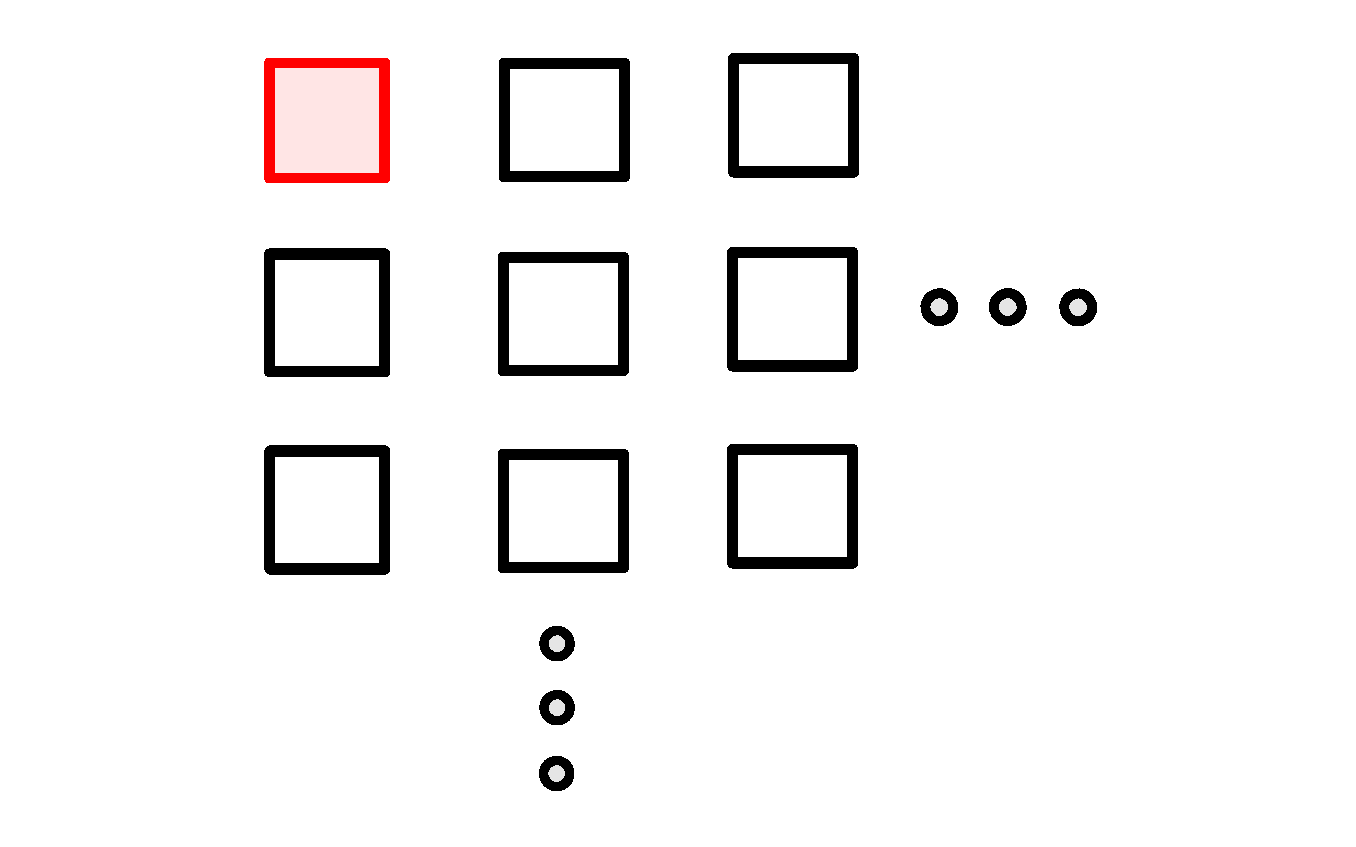
\includegraphics[width=\textwidth]{images/CBN.pdf}
\caption{Example of an Corner Base-Node configuration. The base-node is colored and highlighted in red.}
\end{figure}~\label{fig:cbn}

Here we introduce a particular representation (based on graph-theory) for a tile which is useful for simplifying simulations and for analyzing particular routing configurations.
The most general tile configuration occurs when we assume that all adjacent nodes within the tile are connected; this creates what we refer to as a ``fully connected tile'' (FCT).
An example of a FCT is shown in Figure~\ref{fc_tile}.
Any particular choice of an effective routing must then be a subset of this fully connected version.

\begin{figure}[]
\centering
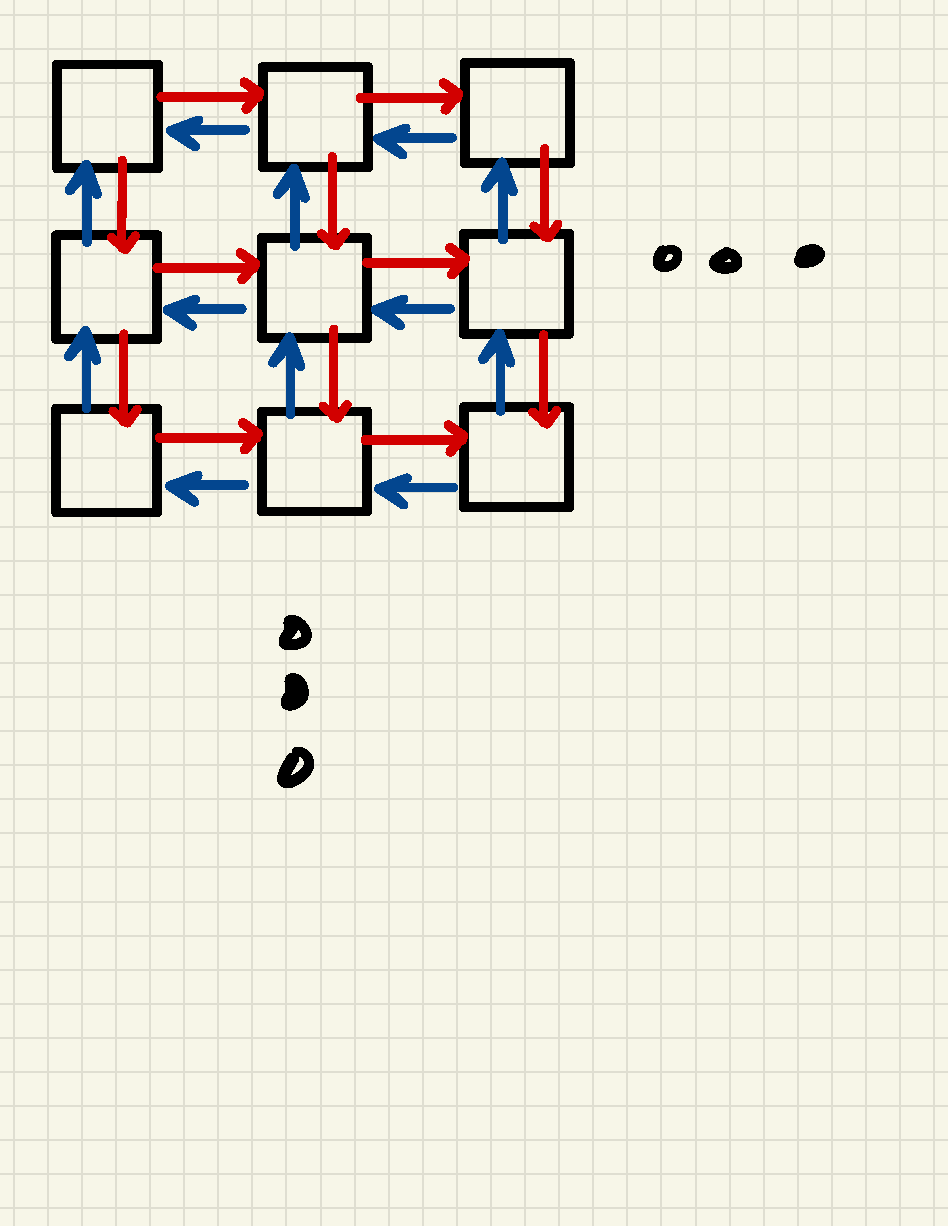
\includegraphics[width=\textwidth]{images/Notes.pdf}
\caption{Example of the fully connected routing configuration for a tile (FCT). Each Node represents a digital channel which must be aggregated, and the red and blue connections distinguish directions of communication. The red connection lines indicate pathways away from the base node, whereas the blue lines represent connection paths towards the base-node in the upper-left.}
\end{figure}~\label{fig:fc_tile}

To elaborate on the adjacency matrix of the FCT we consider an $2\times 3$ tile.
A $2\times 3$ tile has six total nodes, where we consider the upper-left most node to be the base node.
Then, the unweighted adjacency matrix has dimensions $6\times6$ of the form:
\begin{equation}
M =
 \begin{pmatrix}
 0 & 1 & 0 & 1 & 0 & 0 \\
 1 & 0 & 1 & 0 & 1 & 0 \\
 0 & 1 & 0 & 0 & 0 & 1 \\
 1 & 0 & 0 & 0 & 1 & 0 \\
 0 & 1 & 0 & 1 & 0 & 1 \\
 0 & 0 & 1 & 0 & 1 & 0 \\
 \end{pmatrix}
\end{equation}~\label{eq:adjacency_matr}


Where each non-zero value of $M_{ij}$ represents a connection between nodes $i$ and $j$.
As an unweighted, undirected graph this is a symmetric matrix.

In practice each digital channel within a tile is actually controlled by a unique, free-running oscillator.
Therefore, we can define the length of each edge between nodes as the length of time to send of a packet of data between two nodes ($T_{i\rightarrow j}$).
With this we can extend the model the adjacency matrix as a weighted and directed graph if we recognize that the non-zero elements of $M_{ij}$ become $T_{i\rightarrow j}$, or the length of time it takes for the $i^{th}$ local oscillator to transmit a packet to node $j$.

We can generalize this matrix in terms of an arbitrary number of rows ($r$) and columns ($c$).
We define a convention of numbering nodes within the tile in terms of increasing column number followed by increasing row number.
With this convention we obtain the general adjacency matrix with values defined by:
\begin{equation}
  M_{ij} = T_{i\rightarrow j}(\delta_{i,j=i\pm 1} + \delta_{i,j=i\pm r})
\end{equation}~\label{eq:adjacency_comp}

An adjacency list can similarly be constructed from Equation~\ref{eq:adjacency_comp} where the non-zero connections are given by the kroniker-deltas factors.

The length between the nodes represets the time it takes for a packet to transact from one node to the next.
This is determined by both the number of clocks to be sent in the communication protocol ($N_{bits}$) and the period of the transmitting and receiving oscillators, $T_{i}$ and $T_{j}$, respectively.
Unlike the transmitter, the receiver only affects the transaction time with a single clock cycle, as the protocls we test here, (UART and Endeavor), each conclude a packet transaction when the receiver records the last bit transaction from the transmitter.

The full length between two nodes, $i$ and $j$, connected by an edge is represented by:
\begin{equation}
T_{i\rightarrow j} = N_{bits}T_{i} + T_{j}(t)
\end{equation}~\label{eq:t_packet_full}

where $T_{j}(t)$ represents the time dependent fractional part of one nominal clock period of the receiving node.
The expectation value of $T_{j}(t)$ is half of the nominal window so that mean Equation~\ref{eq:t_packet_full} is:
\begin{equation}
\bar{T}_{i\rightarrow j} \simeq N_{bits}T_{i} + \frac{T_{j}}{2}
\end{equation}~\label{eq:t_packet_avg}

Since the transaction time of a packet is much larger than a single clock cycle ($N_{bits} \simeq \mathcal{O}(10^{2}) \gg \frac{1}{2}$), we can approximate Equation~\ref{eq:t_packet_avg}:

\begin{equation}
\bar{T}_{i\rightarrow j} \approx N_{bits}T_{i}
\end{equation}~\label{eq:t_packet}

This representation is also useful to model certain SPF where a node becomes inactive.
Dead or inactive nodes are ones in which all of their connections are effectively disconnected.
This is equivalent to setting their transaction lengths to zero: $T_{SPF} = 0$.

We comment that although it is possible to construct tiles where more than one node connects to the aggregator, we observe that this configuration simply produces two effective tiles.
These distinct tiles then are the data paths which are unique to each base-node.
In this graphical representation a packet of data can follow one, and only one path from the origin node to the base-node unless there was duplication of packets.
We emphatically avoid designs which might depend on data duplication for reduncancy; these two base-nodes are in unconnected graphs.

Additionally, it is possible to connect non-rectangular tiles, but these tiles are effectively a larger rectangular tile with disconnected nodes to produce the desired shape.
Since every node is designed to be robust in the full version, it will be be robust in the subset.

We can apply this same argument to base-nodes which do not lie at the corners of the rectangular tile.
In the case where the base-node is selected along the edge
Therefore, we conclude that the analysis of the tile with the above adjacency matrix and a selection of the base-node at the corner of a rectangular corner provides the basis problem to the tile configuration.

\subsubsection{The SPF Cost}~\label{sec:spf_cost}

We define the average SPF cost as the amount of nodes that will be lost during a transaction as the number of digital channels at a height below the failed digital channel.
For example, the number of nodes which are lost if a leaf-node fails is one since no other channels are between it and the data node.
Likewise, the number of nodes which are lost in the event of a base-node failure is the total tile, $N$.

We can then calculate a mean cost SPF, $C_{SPF}$, :
\begin{equation}
  C_{SPF} = \frac{1}{N}\sum_{node} \frac{n_{i}}{N} = \frac{1}{N^{2}}\sum_{node} n_{i}
\end{equation}~\label{eq:cspf}

\subsubsection{Minimize Occupancy}~\label{sec:min_conn}

One of the goals of a succesful digital design is to ensure lossless data transfer.
One point of failure on the digital side is an overabudance of data arriving at a single layer within the tree.
This data loss occurs when data are sent to a node faster than the data leaves the node, and persists for long enough such that the buffers of the node overflow.
This creates a horrible loss of data which can't be recovered.

A routing scheme which minimizes the overall occupancy in the tree depths is shown in Figure~\ref{fig:snake}.
We refer to the style of routing as ``Snake''-routing (SR), because this is also the longest possible routing scheme for a square tile.

\begin{figure}[]
\centering
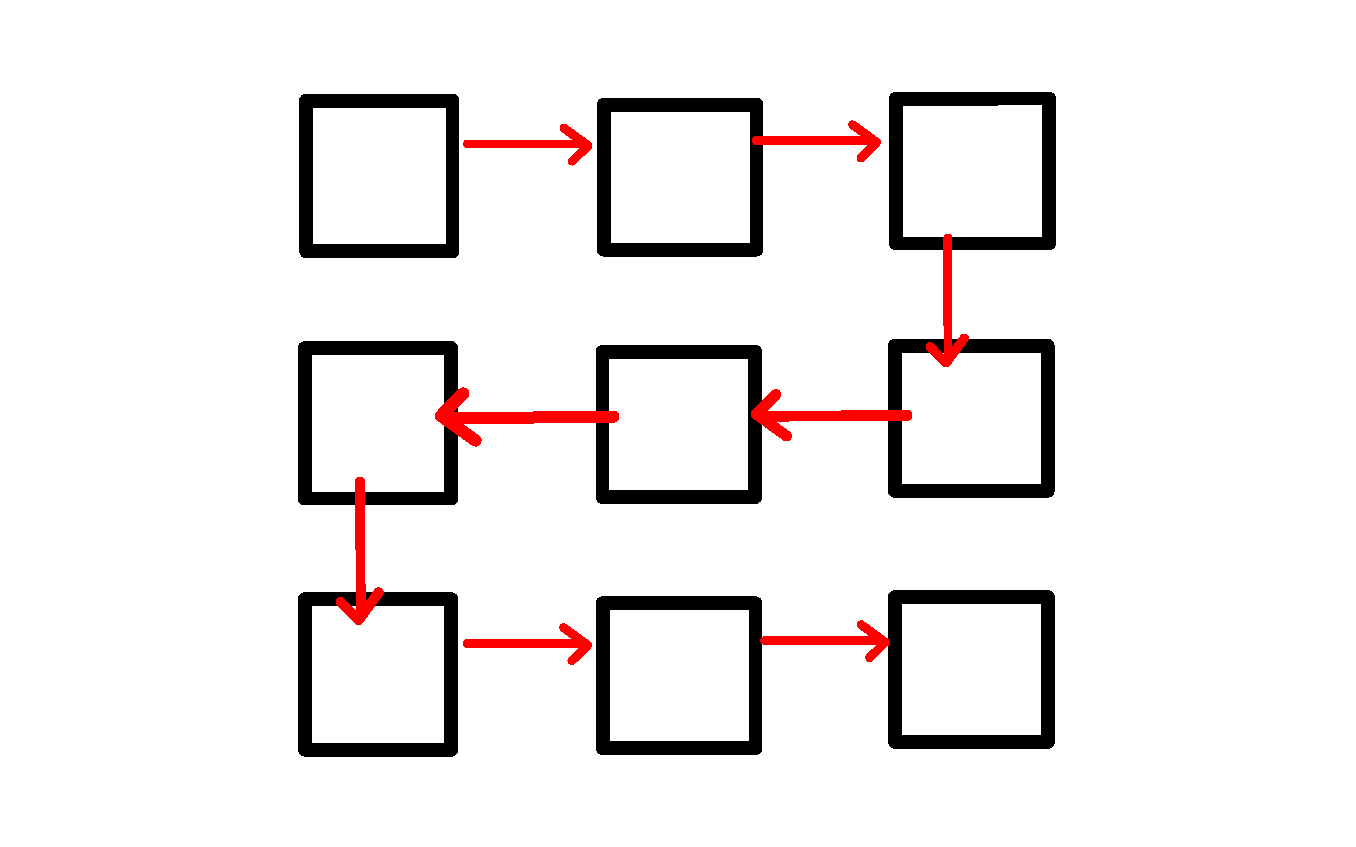
\includegraphics[width=\textwidth]{images/snakeroute.pdf}
\caption{Minimal Occupancy Path of a FCT. This routing path ensures that the number of input connections equal the number of output paths for the node.}
\end{figure}~\label{fig:snake}

We inspect the SPF risk from this routing scheme with Equation~\ref{eq:cspf}, where we notice that the $n_{i}$ of each node is simply a running sum from the leaf to $N$ at the base node.

\begin{equation}
  C_{SPF} = \frac{1}{N^{2}}\frac{N(N+1)}{2} = \frac{1}{n}\frac{N+1}{2} = \frac{1}{2} + \frac{1}{2N}
\end{equation}~\label{eq:cspf_snake}

Equation~\ref{eq:cspf_snake} tells us that the SPF risk of this routing configuration converges to half as the size of the tile grows.
Intuitively, this makes sense, since it is equally likely to select a node close to the base-node as it is far away, which implies that the sum should converge to half the tile size for large $N$.

Although this routing scheme provides the most lax constraint on the requried buffers at each digital channel, it provides the longest average path between the base node.
The longer the transaction delay between the base-node and other nodes increases the reconstruction time uncertainty.
Therefore, a natural alternative routing scheme is one that minimizes the communication scheme.

\subsubsection{Minimize Delay}~\label{sec:min_comm}

For any given node in an edge FCT with location $(R_{i},C_{i}$), the shortest path to the base-node is simply the sum of its coordinates: $R_{i}+C_{i}$.
An example of such a routing configuration for a tile is shown in Figure~\ref{fig:leftroute}.

\begin{figure}[]
\centering
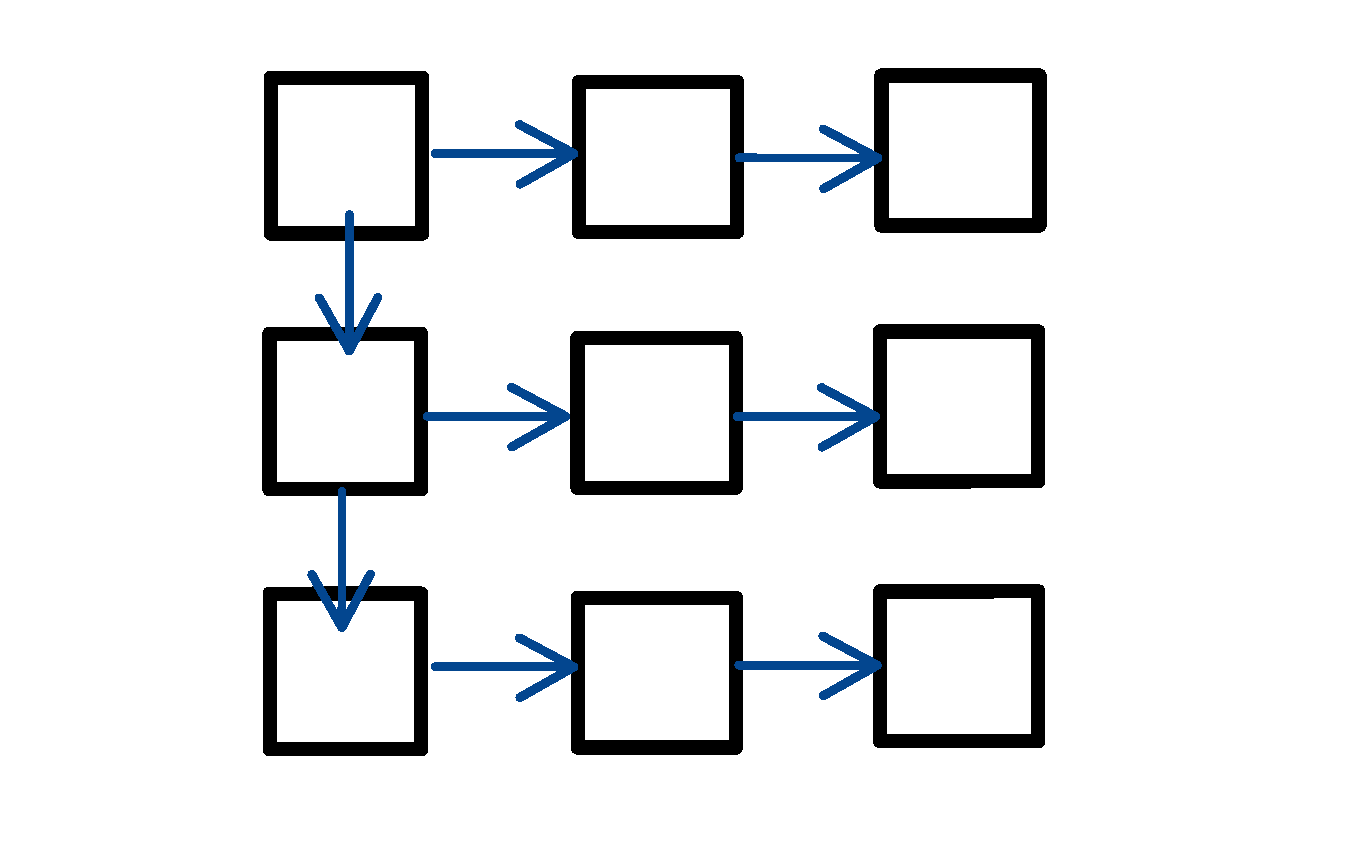
\includegraphics[width=\textwidth]{images/leftroute.pdf}
\caption{Minimal Delay Path of a FCT. This routing path ensures that the minimum number of transactions occur from every node in the FCT to reach the base-node. For any node along any column this is equivalent to the sum of the row and column of that node.}
\end{figure}~\label{fig:leftroute}

We can calculate $C_{SPF}$ for this routing configuration if we identify that there are a $C$ number of rows which sum from one to $R-1$.
Likelise, the far-left column in Figure~\ref{fig:leftroute} shows that the number of rows, $R$, sum from one to $C$.
We can rewrite the sum over all nodes in Equation~\ref{eq:cspf} as:

\begin{equation}
  \sum_{node}n_{i} = C\sum_{i=0}^{i=R-1}i + R\sum_{i=0}^{i=C}i
\end{equation}~\label{eq:cspf_left_s}

We simplify the running sum of each term in Equation~\ref{eq:cspf_left_s}:
\begin{equation}
  \sum_{node}n_{i} = C\frac{R(R-1)}{2} + R\frac{C(C+1)}{2} = RC(\frac{R+C}{2})
\end{equation}~\label{eq:cspf_left_e}

Using this result we obtain $C_{SPF}$ by identifying $N = RC$:
\begin{equation}
  C_{SPF} = \frac{1}{N^{2}}\sum_{node}n_{i} = \boxed{\frac{R+C}{2RC}}
\end{equation}~\label{eq:cspf_left_fin}

This result informs that relative cost of losing a node tends to zero as the size of the tile grows.
Again, this result can be obtained intuitively, since as the number of columns (or rows) grow in size, the probability of a single failure occuring on the aggregator column is increasingly less likely.


\subsubsection{Broadcasts to avoid SPF}~\label{sec:broadcast}

In order to protect against SPF we only consider a designs which implement the FCT, since SPF can occur on any node the most robust connection scheme is the FCT.
A FCT allows searches to probe all possible paths to any node via a ``broadcast'' produced from packets sent by the aggregator to the base-node.
Therefore the broadcast algorithm can be represented by a complete circuit which begins at the base-node and proceeds to a target node with no repeated nodes until the target node is reached.
The backward path is then completed in reverse by following the edges (connections) between each node until arriving finally again at the base-node.

In practice, we encode the broadcast packet with a special header, to differentiate it from a request packet. 
To differentiate broadcasts an identification number is also included in the packet.
Then, any node which receives a broadcast packet will record the identification number of the most recent broadcast, which it uses to discard repeated broadcast packets that arrive with the same identification number.

In the event that a particular node becomes inactive it will ``block'' data comming from the nodes along its path.
In this case, there must be some sort of ``broadcast'' originating from the base-node that would allow information tranverse regardless of the effective routing path.

%% colored matrix
\def\r{\color{red}1}
\def\b{\color{blue}1}
\begin{figure}[h]
  \begin{tabular}{p{5cm}c}
    {${\renewcommand{\arraystretch}{2.0}}
        \begin{pmatrix}
          0 & \r & 0 & \r & 0 & 0 \\
          \b & 0 & \r & 0 & \r & 0 \\
          0 & \b & 0 & 0 & 0 & \r \\
          \b & 0 & 0 & 0 & \r & 0 \\
          0 & \b & 0 & \b & 0 & \r \\
          0 & 0 & \b & 0 & \b & 0 \\
        \end{pmatrix}$}
    &
    $\vcenter{\hbox{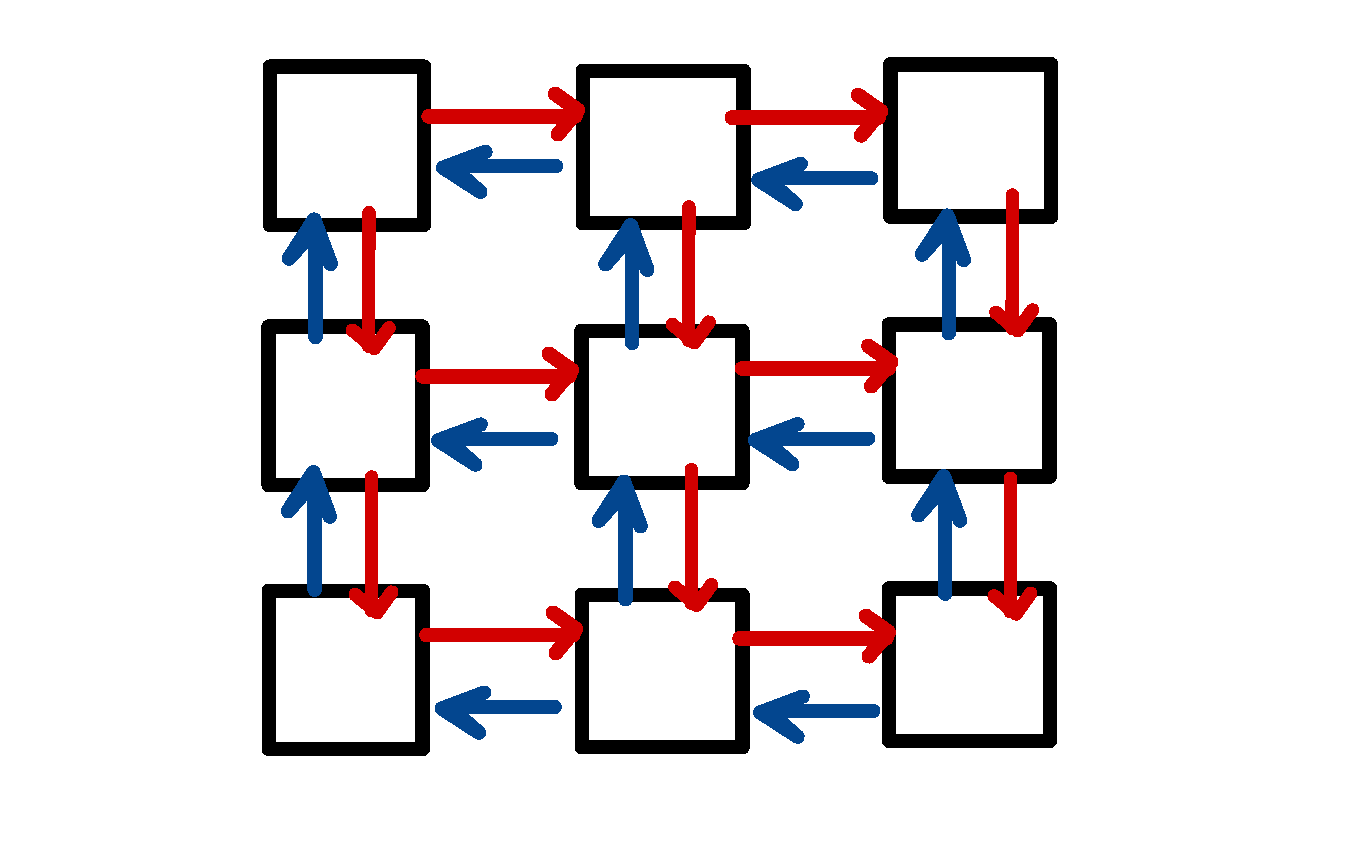
\includegraphics[scale=0.5]{images/Broadcast.pdf}}}$
  \end{tabular}
\caption{Minimal Routing Path of a FCT. This routing path ensures that the number of input connections equal the number of output paths for the node.}
\end{figure}~\label{fig:FCT_colored}

\subsection{Comments on the Edge Base-node and Other Routings}~\label{sec:base_node}

We discuss here the case of a FCT with an edge base node.
An edge base node (EBN) is a digital channel that connects to the aggregator and to three other digital channels within a tile.
Like before, this base-node must provide a unique path during data transmission to all digital channels within the tile.
In this configuration the adjacency matrix is still the same as given in Equation~\ref{eq:adjacency_comp}.

Also, as before, we wish to inspect different routing scenarios for a tile of a given square dimension of $R$ rows and $C$ columns.
We can proceed by dividing the FCT graph into two subgraphs, $S1$ and $S2$, where $S1$ represets the rectangular section of the graph below and to the left of the EBN, while $S2$ are the remaining channels.

We identify that while the number of columns ($C$) in tile is equal to both subgraphs, the total number of rows $R$ of the tile is equal to the sum of the rows from these two subgraphs: $R = R_{1} + R_{2}$.

\begin{figure}[]
\centering
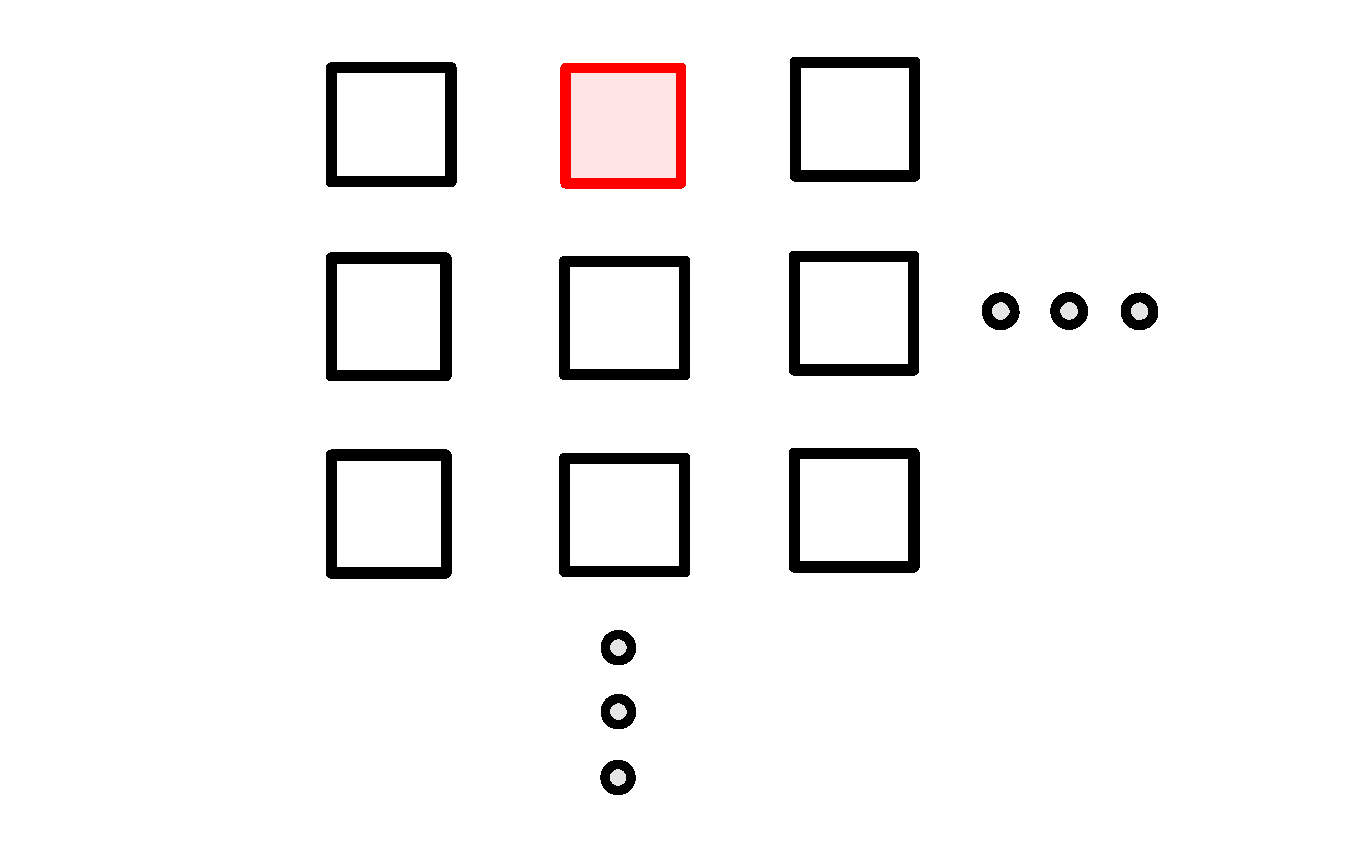
\includegraphics[width=\textwidth]{images/EBN.pdf}
\caption{Example of an Edge base-node configuration. The base-node is colored and highlighted in red.}
\end{figure}~\label{fig:ebn}

% \begin{tikzpicture}[->,>=stealth',shorten >=1pt,auto,node distance=1.25cm,
%                     ,auto=center]
%                     % ,auto=center,every node/.style={circle,fill=blue!20}]
%   \tikzstyle{every node}=[fill=blue,draw=none,text=white]

%   \node (1) at (0,0) {1};
%   %% row 1
%   \node (2) at (1,-1) {2};
%   \node (3) at (2,-2) {3};
%   \node (4) at (3,-3) {4};
%   % row 2
%   \node (5) at (0, -1) {5};
%   \node (6) at (1,-2) {6};
%   \node (7) at (2,-3) {7};
%   \node (8) at (3,-4) {8};

%   %% end nodes
%   \node (10) at (0, -5) {$C$}; % must be at 0 x
%   \node (11) at (5, -5) {$R$}; % must be 1:1 slope
%   \node (12) at (5, -10) {$R+C$}; % must be 1:1 slope

%   %% paths
%   % \path (4) -- (11) [red, midway, sloped] {$\dots$};
%   % \path (5) -- (10) [red, midway, sloped] {$\dots$};
%   \draw[red,thick,dashed] (4) -- (11);
%   \draw[red,thick,dashed] (5) -- (10);
%   \draw[red,thick,dashed] (10) -- (12);
%   \draw[red,thick,dashed] (11) -- (12);

%   \path (1) edge (2);
%   \path (1) edge (5);
%   \path (2) edge (3);
%   \path (3) edge (4);
%   \path (5) edge (6);
%   \path (6) edge (7);
%   \path (7) edge (8);
% \end{tikzpicture}

The EBN then is actually just a composition of two subgraphs which are each equivalent to The tree characteristics which determine requirements for the digital channels are the tree height and total occupancy at each level.
Therefore, since the EBN provides no difference in either of these characteristics and is a suposition of two fundamental CBN, an analysis of an EBN is equivalent to the analysis of a CBN.

However, we do remark comment that the average difference of the relative weights of each node in a SPF analysis are different in a EBN compared to the CBN case.
This should be obvious since the relative weight of each node is determined by the running sum of the path length betwee the base-node and its leaf.
For a fixed row dimension, $R$, the EBN offers a smaller average tree height for each of its componet radia $R_{1}$ and $R_{2}$.

Therefore, in a EBN tile, with two subgraphs of radii $R_{1}$ and $R_{2}$ where the base-node is on the $R_{1}$ edge.
The total sum of the weights of all nodes in the tile are the sums of the two subgraphs plus $CR_{2}$, which is the average weight of the nodes from the subgraph $R_{2}$ when it connects to $R_{1}$.
\begin{equation}
  \sum_{node}n_{i} = \sum_{R_{1}} + \sum_{R_{2}} + CR_{2}
\end{equation}~\label{eq:cspf_ebn}

Equation~\ref{eq:cspf_ebn} gives the general formula for calculating the SPF risk for a EBN case, depending on the routing methods of subgraphs $R_{1}$ and $R_{2}$.
We can treat these sub-graphs as in equation~\ref{eq:cspf_left_fin} to obtain:
\begin{equation}
  \sum_{R_{1}} + \sum_{R_{2}} + CR_{2} = \frac{R_{1}C(R_{1}+C)}{2} + \frac{R_{2}C(R_{2}+C)}{2} + CR_{2}
\end{equation}~\label{eq:cspf_e}

We use this result to obtain the relation of the general $C_{SPF}$:
\begin{equation}
  C_{SPF} = \frac{1}{N^{2}}(\frac{R_{1}C(R_{1}+C)}{2} + \frac{R_{2}C(R_{2}+C)}{2} + CR_{2})
\end{equation}

if we identify that $N = C(R_{1}+R_{2})$ and use $R_{2} = R - R_{1}$:
\begin{equation}
  C_{SPF} = \frac{1}{2CR^{2}}(2R_{1}^{2}-2R_{1}R+R^{2}+CR+2(R-R_{1}))
\end{equation}


\section{Frequency Calibration of Local Oscillators}~\label{sec:calib}

The Q-Pix calibration requirements are described in detail in Section~\ref{sec:qpix_calib}.
The important parameters which must be calibrated for each pixel are the charge per reset and the frequency of the local oscillator.
An aim of this work is to demonstrate an additional frequency calibration method using the minimal required connections between each digital node.

Any method of a frequency calibration must synchronize time measurements between all digital nodes within a tile and the aggregator.
There are several possibile methods to achieve this, but ultimately the data that are recorded must be some time at the aggregator, $T_{a}$, and the time at any specific node, $T_{j}$.

%% distribute clock for calibration of time
A direct method is one where the aggregator distributes its own clock to all nodes in the tile.
This scenario removes the need for a calculation of the frequency of each node altogether since the clock of each node is already known from the aggregator.
This is the simplest case for timing calibration: remove all free running oscillators.
However, this method also introduces complex routing and power requirements within every tile.

% TODO
% cross-talk
A distributed clock network indeed removes ambiguity of the remote oscillator frequencies, but at the cost of hardware complexity.
Whether or not this design choice is preferred is entirely detector dependent, but likely increases in difficulty with the scale of the TPC.

We comment, however, that we ignore this scenario because it may altogether be unnecessary depending on future ASIC performance.
In the event that frequency calibrations of sufficient precision ($\bar{f} \approx 1 ppm$) are possible occur on free-running local oscillators future detectors would need only to acquire these ASICs and place them with minimal cost in terms of both time and money.

%% distribute trigger for calibration of time
Another simple scenario is one where the aggregator itself connects directly to all nodes within a tile via a single connection which can be used as a reference trigger.
This means that some trigger from the aggregator would issue directly into each node at the same time: $T_{a} = T_{n}$.
To calcuate the frequency in this manner, the controller would issue two triggers from the aggregator with a known time separation, $T_{o} = T_{a2} - T_{a1}$.
The remote nodes would each record and send their timestamps back to the aggregator, where the time difference would be calculated as:

\begin{equation}
  T_{o} = T_{a2} - T_{a1} = T_{n2} - T_{n1}
\end{equation}

this is rewritten in terms of frequency as follows:
\begin{equation}
  f_{n} = \frac{T_{n2} - T_{n1}}{T_{o}}
\end{equation}

This calibration method extremely simple but introduces an additional connection to each node between itself and the aggregator.
For a large scale system such as Q-Pix even this simple connection scheme introduces $\approx 60\times 10^{3}$ hardware points of failure per APA.

Both of these scenarios are valid implementations of a Q-Pix readout system.
In both of these scenarios, however, there is added complexity into the hardware design of the system in the form of additional routing where each route which represents a possible point of failure.

In a world of perfect hardware and costless routing in terms of both time and money these routing schemes would clearly be sufficient.
However, no hardware is perfect.
Therefore we introduce and discuss a calibration technique which relies on no additional routing and could be optionally implemented even in the above schemes in the event of a failure.
Therefore, even if not the primary implemented calibration technqiue, since this calibration introduces no superfluous routing it could still be used regardless of the actual future hardware implementation.

%% distribute packet for calibration of time
\subsection{A Minimal Connection Calibration Procedure}~\label{sec:min_calib}

As stated in the previous section, any frequency calibration records a reference time at the aggregator ($T_{a}$) and an event time ($T_{n}$) at a node within a tile.

the time calibration procedure presented here requires only the minimal routing required in any Q-Pix readout system, where we assume time-dependent free-running local oscillators at each node within the tile.

%% issue 1
The calibration procedure begins at a time ($T_{0}$) where the aggregator sends a calibration packet.

%% recv1
Next, the packet propagates through the tile to some remote node, $N_{j}$.
This node receives the packet later at some time $T_{n1}$:

\begin{equation}
  T_{n1} = T_{o} + T_{f1}
\end{equation}

Where $T_{f1}$ is the propogation time of the packet from the aggregator to the $N_{j}$ node.

%% meas1
This remote node then sends the packet with its time ($T_{n1}$) back to the aggregator.

%% wait
The aggregator will wait some calibration time ($T_{cal}$) before issuing another calibration packet.
This wait period $(\mathcal{O}(10^{0-2})$) can be long compared to the full transaction time to the $N_{j}$ node $(\mathcal{O}(j*10^{-5})$).

%% issue 1
After the wait period, the aggregator will issue a second calibration packet to be sent to a remote node at time:
\begin{equation}
  T_{1} = T_{cal} + T_{0}
\end{equation}

%% recv2 and meas2
Similarly to the first packet this packet will propagate to $N_{j}$ with some new time $T_{f2}$ where $N_{j}$ will record time $T_{n2}$:
\begin{equation}
  T_{n2} = T_{1} + T_{f2}
\end{equation}

Now, we define $\Delta T_{j}$ as the difference in the two time measurements from the two packets sent from the aggregator.
The time difference is related to the number of clocks that occured between the two different measured values of the clock, $T_{n1}$ and $T_{n2}$.

\begin{equation}
  \Delta T_{j} = T_{n2} - T_{n1}
\end{equation}

We use the known relationships for $T_{n2}$ and $T_{n1}$ to obtain:
\begin{equation}
  \Delta T_{j} = (T_{1} + T_{f2}) - (T_{o} + T_{f1}) = (T_{1} - T_{0}) + (T_{f2} - T_{f1}) = T_{cal} + \Delta T_{f}
\end{equation}

Where we defined $\Delta T_{f}$ as the difference in forward propagation times from the packets sent from the aggregator node at $T_{1}$ and $T_{0}$.

We arrive at the result which compares the measured time at the aggregator $T_{cal}$ and the time measured at each node, $\Delta T_{j}$:
\begin{equation}
  \Delta T_{j} = T_{cal} + \Delta T_{f}
\end{equation}

A perfect reconstruction of the nodal frequency would follow if $\Delta T_{f} = 0$.
But it is sufficient to note that the wait period happens on the order of seconds, whereas $\Delta T_{f}$ is on the order of $\mu s$ or at least a six order of magnitude difference.
We then use $\Delta T_{f} \ll T_{cal}$ to obtain:
\begin{equation}
  \Delta T_{j} \approx T_{cal}
\end{equation}

We convert time into frequency with the difference of the timestamps measured and a known aggregator frequency ($f_{a}$):
\begin{equation}
   \frac{\Delta N_{j}}{f_{j}} = \frac{\Delta N_{a}}{f_{a}}
\end{equation}

or,
\begin{equation}
   \boxed{f_{j} = \frac{\Delta N_{j}}{\Delta N_{a}}f_{a}}
\end{equation}

Where $\Delta N_{j}$ and $\Delta N_{a}$ are the differences in the timestamps of the 32-bit clocks at the remote node and aggregator, respectively.


\subsubsection{Packet Transaction Time}

 We next examine the approximation that $\Delta T_{f} \ll T_{cal}$ and consider its contribution to the error in the reconstruction of $T_{j}$.
This analysis also provides a constraint on the duration of $T_{cal}$ to ensure an accurate measurement of each $T_{j}$ in a tile.
We begin by discussing how long it takes for a packet to traverse a tile.

The time it takes for each packet to be received by the next node is given in Equation~\ref{eq:t_packet}.
The value, $N_{bit}$, is the number of clock cycles used for the packet and is protocol-dependent.
Since the protocol must be deterministic for each packet, $N_{bits}$ must be the same for each transaction on the path from the base-node to the remote node.

As an example, the time it takes for a packet to go from the base-node, $N_{1}$, to a remote node, $N_{3}$, via the path $1\rightarrow 2 \rightarrow 3$ is determined by:
%% packet transaction time
\begin{equation}
  T_{1\rightarrow 3} = T_{1\rightarrow 2} + T_{2\rightarrow 3} \approx \frac{N_{bits}}{f_{1}} + \frac{N_{bits}}{f_{2}} = N_{bits}(\frac{1}{f_{1}} + \frac{1}{f_{2}})
\end{equation}~\label{eq:t_packetTransfer}

Where, $f_{i}$, is the frequency of the clock at sending node. The approximation is within a single clock cycle of the receiving digital node ($\approx 33~\unit{ns}$).

Therefore the time it takes for a packet for go from the base-node to any remote node is proportional to $N_{bits}$ multiplied by the sum of the edges in the full adjacency matrix given by Equation~\ref{eq:adjacency_comp}.

We generalize Equation~\ref{eq:t_packetTransfer} to represent the time it takes a packet to go from the aggregator ($i = 0$) to any remote node, $N_{j}$:
\begin{equation}
  T_{f} = T_{0\rightarrow j} = N_{bits}\sum_{i=0}^{i=j-1}\frac{1}{f_{i}}
\end{equation}

We require that every calibration packet on the protocol uses the same number of clocks ($N_{bits}$ is constant) and follows the same path. $\Delta T_{f}$ becomes:
\begin{equation}
  \Delta T_{f} = N_{bits}\sum_{i=0}^{i=j-1}\frac{1}{\Delta f_{i}} = N_{bits} \sum_{i=0}^{i=j-1}\Delta T_{i}
\end{equation}

We recognize $\Delta T_{i}$ as the nominal time-dependent clock drift of the each local oscillator in the path between the base-node to the remote-node.
We can provide an order of magnitude estimate for $\Delta T_{f}$ if we assume a (very poor) $\approx 1\%$ drift in each of the remote clocks within the tile during a period of $T_{cal} \approx 1~\unit{s}$.
In this approximation we also assume that the mean of the periods of the nodes are the designed value ($\approx 33~\unit{ns}$) for which a 1\% error gives $\sigma_{T_{f}} \approx 3~\unit{ps}$.
If we assume that all of the clocks (for whatever reason) drift have error which drifts int he same direction (the sum doesn't cancel) then for 100 transactions with 1000 clocks per transaction, we obtain for $\Delta T_{f}$:
\begin{equation}
  \Delta T_{f} \approx 1000 * 100 * 3\times 10^{-12} \approx 30~\unit{ns} \ll 1~\unit{s} \simeq T_{cal}
\end{equation}
